
% Q16
\question In the figure, $OAB$ and $OCD$ are sectors with centre $O$ . If $\wideparen{AB} = 12\pi\text{ cm}$ , $\wideparen{CD} = 16\pi\text{ cm}$ and $OA = 30\text{ cm}$ , then $AC =$

\begin{minipage}{0.45\textwidth}
\begin{choices}
    \choice $5\text{ cm}$ .
    \correctchoice $10\text{ cm}$ .
    \choice $20\text{ cm}$ .
    \choice $40\text{ cm}$ .
\end{choices}
\end{minipage}
\begin{minipage}{0.52\textwidth}
\centering
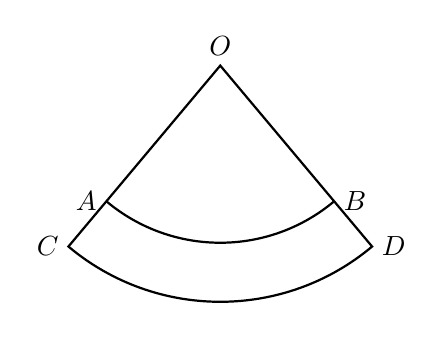
\begin{tikzpicture}[scale=0.075]
    \coordinate (O) at (0,0);
    \draw[thick] (O) -- (-130:40) arc (-130:-50:40) -- cycle;
    \draw[thick] (-130:30) arc (-130:-50:30);
    \node[above] at (O) {$O$};
    \node[left] at (-130:30) {$A$};
    \node[right] at (-50:30) {$B$};
    \node[left] at (-130:40) {$C$};
    \node[right] at (-50:40) {$D$};
\end{tikzpicture}
\end{minipage}
\begin{solution}
\[ \frac{OC}{OA} = \frac{\widehat{CD}}{\widehat{AB}} \implies \frac{30 + AC}{30} = \frac{16\pi}{12\pi} = \frac{4}{3} \implies 30 + AC = 40 \implies AC = 10\text{ cm} \quad \text{(B)} \]
\end{solution}

% Q17
\question In the figure, $ABCD$ is a parallelogram. $E$ and $F$ are points lying on $AB$ and $CD$ respectively. $AD$ produced and $EF$ produced meet at $G$ . It is given that $DF : FC = 3 : 4$ and $AD : DG = 1 : 1$ . If the area of $\triangle DFG$ is $3\text{ cm}^2$ , then the area of the parallelogram $ABCD$ is

\begin{minipage}{0.45\textwidth}
\begin{choices}
    \choice $12\text{ cm}^2$ .
    \correctchoice $14\text{ cm}^2$ .
    \choice $18\text{ cm}^2$ .
    \choice $21\text{ cm}^2$ .
\end{choices}
\end{minipage}
\begin{minipage}{0.52\textwidth}
\centering
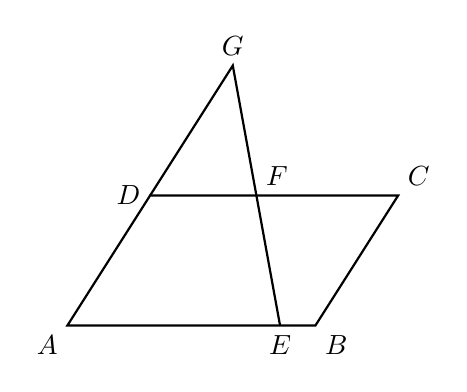
\begin{tikzpicture}[scale=0.75]
    \coordinate (A) at (0,0);
    \coordinate (B) at (4.2,0);
    \coordinate (D) at (1.4,2.2);
    \coordinate (C) at (5.6,2.2);
    \coordinate (G) at (2.8,4.4);
    \coordinate (F) at (3.2,2.2);
    \coordinate (E) at (3.6,0);
    \draw[thick] (A) -- (B) -- (C) -- (D) -- cycle;
    \draw[thick] (D) -- (G) -- (E);
    \node[below left] at (A) {$A$};
    \node[below] at (E) {$E$};
    \node[below right] at (B) {$B$};
    \node[above right] at (C) {$C$};
    \node[above right] at (F) {$F$};
    \node[left] at (D) {$D$};
    \node[above] at (G) {$G$};
\end{tikzpicture}
\end{minipage}
\begin{solution}
Since $\triangle GDF \sim \triangle GAE$ with $GD : GA = 1 : 2$, we have $AE = 2DF$ and $\text{Area}(\triangle GAE) = 4(3) = 12\text{ cm}^2$, so $\text{Area}(ADFE) = 12 - 3 = 9\text{ cm}^2$. \\
Since $DF : FC = 3 : 4$, let $DF = 3k$, $CD = AB = 7k$, and $AE = 6k$. \\
Comparing the sum of parallel bases of trapezium $ADFE$ ($3k + 6k = 9k$) and parallelogram $ABCD$ ($7k + 7k = 14k$) with the same height:
\[ \text{Area}(ABCD) = 9 \times \frac{14}{9} = 14\text{ cm}^2 \quad \text{(B)} \]
\end{solution}

% Q21
\question In the figure, $AB$ is a diameter of the circle $ABCD$ . If $AB = 12\text{ cm}$ and $CD = 6\text{ cm}$ , then the area of the shaded region is

\begin{minipage}{0.45\textwidth}
\begin{choices}
    \choice $(12\pi - 9)\text{ cm}^2$ .
    \choice $(12\pi + 9)\text{ cm}^2$ .
    \choice $(12\pi - 9\sqrt{3})\text{ cm}^2$ .
    \correctchoice $(12\pi + 9\sqrt{3})\text{ cm}^2$ .
\end{choices}
\end{minipage}
\begin{minipage}{0.52\textwidth}
\centering
\begin{tikzpicture}[scale=0.35]
    \def\R{6}
    \coordinate (O) at (0,0);
    \coordinate (A) at (198:\R);
    \coordinate (B) at (18:\R);
    \coordinate (D) at (-100:\R);
    \coordinate (C) at (-40:\R);
    \fill[pattern=north east lines] (A) -- (B) arc (18:-40:\R) -- (D) arc (-100:-162:\R) -- cycle;
    \draw[thick] (O) circle (\R);
    \draw[thick] (A) -- (B);
    \draw[thick] (D) -- (C);
    \node[left] at (A) {$A$};
    \node[right] at (B) {$B$};
    \node[below right] at (C) {$C$};
    \node[below left] at (D) {$D$};
\end{tikzpicture}
\end{minipage}
\begin{solution}
Let $O$ be the centre of the circle ($OA = OB = OC = OD = 6\text{ cm}$). Since $CD = 6\text{ cm}$, $\triangle OCD$ is equilateral ($\angle COD = 60^\circ$). \\
The area of the minor segment cut off by chord $CD$ is $\pi(6)^2\left(\frac{60^\circ}{360^\circ}\right) - \frac{\sqrt{3}}{4}(6)^2 = 6\pi - 9\sqrt{3}\text{ cm}^2$. \\
Subtracting this from the area of the semicircle ($\frac{1}{2}\pi(6)^2 = 18\pi\text{ cm}^2$) gives $(12\pi + 9\sqrt{3})\text{ cm}^2$ (D).
\end{solution}